\documentclass[11pt,a4paper]{article}

\usepackage[utf8]{inputenc}
\usepackage[T1]{fontenc}
\IfFileExists{slovene.ldf}{\usepackage[slovene]{babel}}{}
\usepackage{lmodern}
\usepackage[margin=2.5cm]{geometry}
\usepackage{graphicx}
\usepackage{caption}
\usepackage{float}
\usepackage{booktabs}
\usepackage{tabularx}
\usepackage{enumitem}
\usepackage{xcolor}
\usepackage[hidelinks]{hyperref}
\usepackage{xurl}

\AtBeginDocument{%
  \renewcommand{\figurename}{Slika}%
  \renewcommand{\tablename}{Tabela}%
  \renewcommand{\contentsname}{Kazalo}%
  \renewcommand{\refname}{Viri}%
}

\graphicspath{{slike/}}
\setlist{itemsep=2pt, topsep=4pt}

\title{\textbf{Pekarna Zrno}\\[4pt]
\large Pregled obstoječih rešitev}
\author{
  Val Špiljar \and
  Vid Ekart \and
  Kris Škerget 
}
\date{Maribor, 24.\ november 2026}

\begin{document}

\maketitle
\thispagestyle{empty}

\begin{center}
\small Univerza v Mariboru \\
Predmet: um-KIDS \quad -- \quad Naloga 6: Priprava na razvoj (1.\ del)
\end{center}

\vspace{1em}
\tableofcontents
\newpage

%=====================================================================
\section{Uvod}
%=====================================================================

Pekarna Zrno je družinska pekarna, ki jo je leta 2015 v Mariboru ustanovila
družina s tremi generacijami peke. Začela je z majhno pekarno v središču mesta,
danes pa ima tri poslovalnice in redne stranke po vsej Štajerski. Ponuja kruh iz
drožja, polnozrnati in pirin kruh, sladko in slano pecivo (rogljiči, burek,
štručke), torte in sladice po naročilu ter dostavo za podjetja in dogodke.

\subsection*{Problem}
Pekarna danes nima spletne rešitve za naročanje. Torte in sladice po naročilu ter
dostave za podjetja se urejajo po telefonu ali osebno, kar vodi v:
\begin{itemize}
  \item izgubljena ali napačno zapisana naročila,
  \item slab pregled nad tem, koliko izdelkov je treba speči za naslednji dan,
  \item omejen doseg -- stranke ne morejo preveriti ponudbe, cen ali alergenov,
        ne da bi prišle v poslovalnico,
  \item ostanke neprodanega peciva ob koncu dneva.
\end{itemize}

\subsection*{Naša rešitev}
Razvili bomo spletno aplikacijo za Pekarno Zrno, ki bo strankam omogočala pregled
ponudbe, naročilo izdelkov z izbiro prevzema v eni od poslovalnic ali dostave,
naročanje tort po meri ter posebna (ponavljajoča se) naročila za podjetja. Pekarni
bo aplikacija ponudila pregled naročil po dnevih in poslovalnicah.

Da bi ugotovili, kaj se na trgu že obnese in kje so vrzeli, smo pregledali tri
obstoječe rešitve: spletno trgovino \emph{Pekarne Pečjak}, dostavno platformo
\emph{Wolt} in aplikacijo \emph{Too Good To Go}.

%=====================================================================
\section{Pregled obstoječih rešitev}
%=====================================================================

%---------------------------------------------------------------------
\subsection{Spletna trgovina Pekarne Pečjak}
%---------------------------------------------------------------------

\paragraph{Opis.}
Pekarna Pečjak je slovensko družinsko podjetje, ki ga je leta 1972 na Vrhniki
ustanovil Stanislav Pečjak in je danes eno vodilnih slovenskih podjetij za
proizvodnjo pekovskih in zamrznjenih izdelkov~\cite{pecjak-zgodba}. Na svoji
spletni strani ima lastno spletno trgovino, v kateri je mogoče kupiti bureke,
rogljiče, pecivo, sladice in keks~\cite{pecjak-trgovina}. Je najbližji primer
tega, kar želimo zgraditi: pekarna, ki prodaja neposredno prek lastne strani.

\paragraph{Ključne funkcionalnosti.}
\begin{itemize}
  \item katalog izdelkov po kategorijah (burek, rogljiči, navihanci \dots)
        s filtri in razvrščanjem,
  \item košarica s prikazom, koliko še manjka do brezplačne dostave
        (nad 60\,€)~\cite{pecjak-trgovina},
  \item izbira dostave ali osebnega prevzema na prevzemnih mestih,
        poleg tega t.\,i.\ potujoča trgovina~\cite{pecjak-domov},
  \item uporabniški račun in akcijska ponudba (popusti na izbrane izdelke),
  \item podrobna stran izdelka s sestavinami, alergeni in oznakami
        (npr.\ vegansko),
  \item katalog izdelkov v obliki PDF za prenos.
\end{itemize}

\paragraph{Prednosti.}
\begin{itemize}
  \item lastna blagovna znamka in neposreden stik s stranko (brez provizij
        posrednikov),
  \item pregleden prikaz alergenov in sestavin,
  \item jasen motivator za večje naročilo (prag za brezplačno dostavo),
  \item več načinov prevzema.
\end{itemize}

\paragraph{Slabosti.}
\begin{itemize}
  \item ponudba je usmerjena predvsem v zamrznjene in pakirane izdelke,
        ne v svež kruh za isti dan,
  \item ni naročanja tort ali izdelkov po meri,
  \item na strani nismo zasledili posebne poti za podjetja (redne,
        ponavljajoče se dostave).
\end{itemize}

\begin{figure}[H]
  \centering
  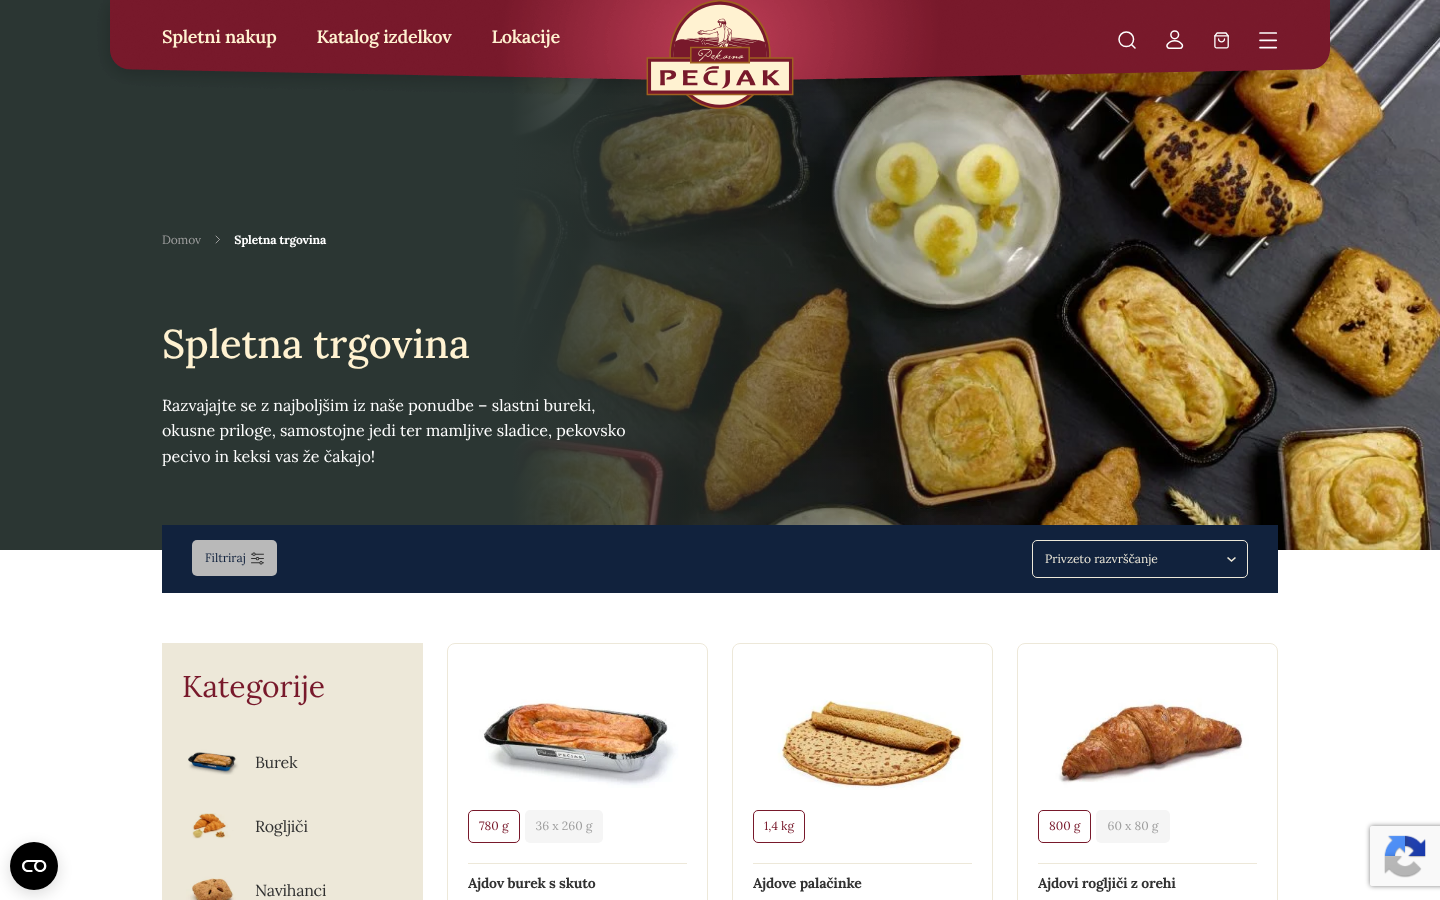
\includegraphics[width=0.92\textwidth]{pecjak_trgovina.png}
  \caption{Spletna trgovina Pekarne Pečjak: kategorije izdelkov, filtri in
  razvrščanje~\cite{pecjak-trgovina}.}
  \label{fig:pecjak}
\end{figure}

%---------------------------------------------------------------------
\subsection{Wolt}
%---------------------------------------------------------------------

\paragraph{Opis.}
Wolt je platforma za dostavo hrane in drugih izdelkov, ki v Sloveniji deluje
tudi v Mariboru~\cite{wolt-kariere}. Na njej so med drugim prisotne pekarne,
kot sta Mlinar in Žito~\cite{wolt-maribor}. Za pekarno pomeni Wolt hiter
način, da pride do strank, ki želijo pecivo dostavljeno na dom ali v pisarno,
brez lastne dostavne službe.

\paragraph{Ključne funkcionalnosti.}
\begin{itemize}
  \item seznam ponudnikov glede na lokacijo, z oceno, ocenjenim časom dostave
        in stroškom dostave,
  \item stran ponudnika z menijem po kategorijah (npr.\ pri Mlinarju: kava,
        sveže pecivo, sendviči, torte, bureki), iskalnikom in seznamom
        alergenov~\cite{wolt-mlinar},
  \item minimalni znesek naročila in prikaz delovnega časa,
  \item \emph{načrtovano naročilo} -- naročilo za kasnejši termin, ko je
        ponudnik zaprt~\cite{wolt-mlinar-brand},
  \item spremljanje dostave v živo, plačilo v aplikaciji, ocene,
  \item storitev \emph{Wolt for Work} za naročila podjetij~\cite{wolt-storitve}.
\end{itemize}

\paragraph{Prednosti.}
\begin{itemize}
  \item zelo hitra dostava (pogosto v 15--25 minutah),
  \item velika obstoječa baza uporabnikov in zaupanje v plačilni sistem,
  \item dovršena uporabniška izkušnja (iskanje, filtri, sledenje),
  \item pekarni ni treba organizirati lastne dostave.
\end{itemize}

\paragraph{Slabosti.}
\begin{itemize}
  \item pekarna plačuje provizijo platformi in nima lastnih podatkov o strankah,
  \item blagovna znamka pekarne je le ena izmed mnogih -- konkurenca je
        oddaljena en klik,
  \item ni primerno za torte po meri ali večja naročila za dogodke,
  \item dostava je omejena na območja, ki jih Wolt pokriva.
\end{itemize}

\begin{figure}[H]
  \centering
  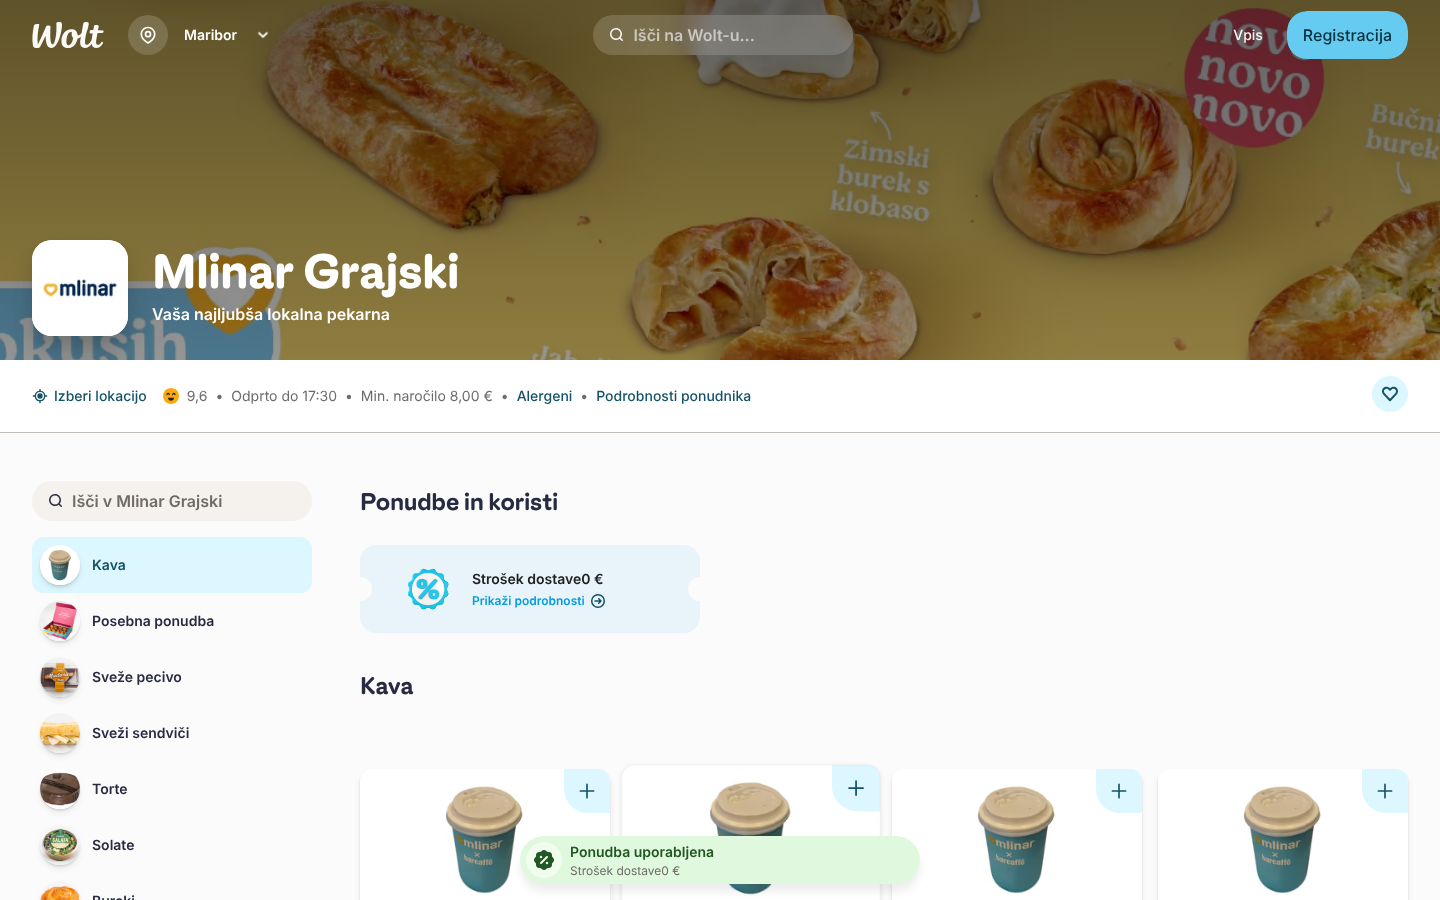
\includegraphics[width=0.92\textwidth]{wolt_mlinar.png}
  \caption{Pekarna Mlinar Grajski na platformi Wolt v Mariboru: ocena,
  minimalni znesek naročila, alergeni in kategorije
  menija~\cite{wolt-mlinar}.}
  \label{fig:wolt}
\end{figure}

%---------------------------------------------------------------------
\subsection{Too Good To Go}
%---------------------------------------------------------------------

\paragraph{Opis.}
Too Good To Go je mobilna aplikacija, ki povezuje uporabnike s pekarnami,
restavracijami in trgovinami, ki imajo ob koncu dneva neprodano hrano.
Uporabnik na zemljevidu najde ponudnike v bližini, rezervira
\emph{vrečko presenečenja} po polovični ceni ali manj in jo ob določenem
terminu prevzame v trgovini~\cite{tgtg-appstore}. Podjetje navaja okoli
100 milijonov registriranih uporabnikov in 170\,000 partnerjev v 19
državah~\cite{tgtg-cz}. Ob pregledu (24.\,11.\,2026) aplikacija v slovenski
različici trgovine App Store ni bila na voljo.

\paragraph{Ključne funkcionalnosti.}
\begin{itemize}
  \item zemljevid in seznam ponudnikov v bližini s kategorijami
        (pecivo, kruh, obroki \dots),
  \item rezervacija in plačilo vrečke presenečenja v aplikaciji,
  \item časovno okno za prevzem (npr.\ 19:30--20:00),
  \item ocene ponudnikov (izkušnja ob prevzemu, kakovost hrane),
  \item poslovni vmesnik za ponudnike, kjer vsak dan nastavijo število
        vrečk~\cite{tgtg-bakery}.
\end{itemize}

\paragraph{Prednosti.}
\begin{itemize}
  \item zmanjša odpadke in pekarni prinese prihodek od izdelkov, ki bi sicer
        šli v smeti,
  \item privabi nove stranke, ki se lahko vrnejo tudi po redno ponudbo,
  \item preprost postopek: rezerviraj, plačaj, prevzemi,
  \item pozitivna podoba trajnostno naravnanega podjetja.
\end{itemize}

\paragraph{Slabosti.}
\begin{itemize}
  \item stranka ne ve natančno, kaj bo v vrečki (problem pri alergijah),
  \item pokriva le ostanke, ne pa rednega naročanja,
  \item v Sloveniji trenutno ni na voljo,
  \item ponudnik od vsake prodane vrečke del zneska prepusti platformi.
\end{itemize}

\begin{figure}[H]
  \centering
  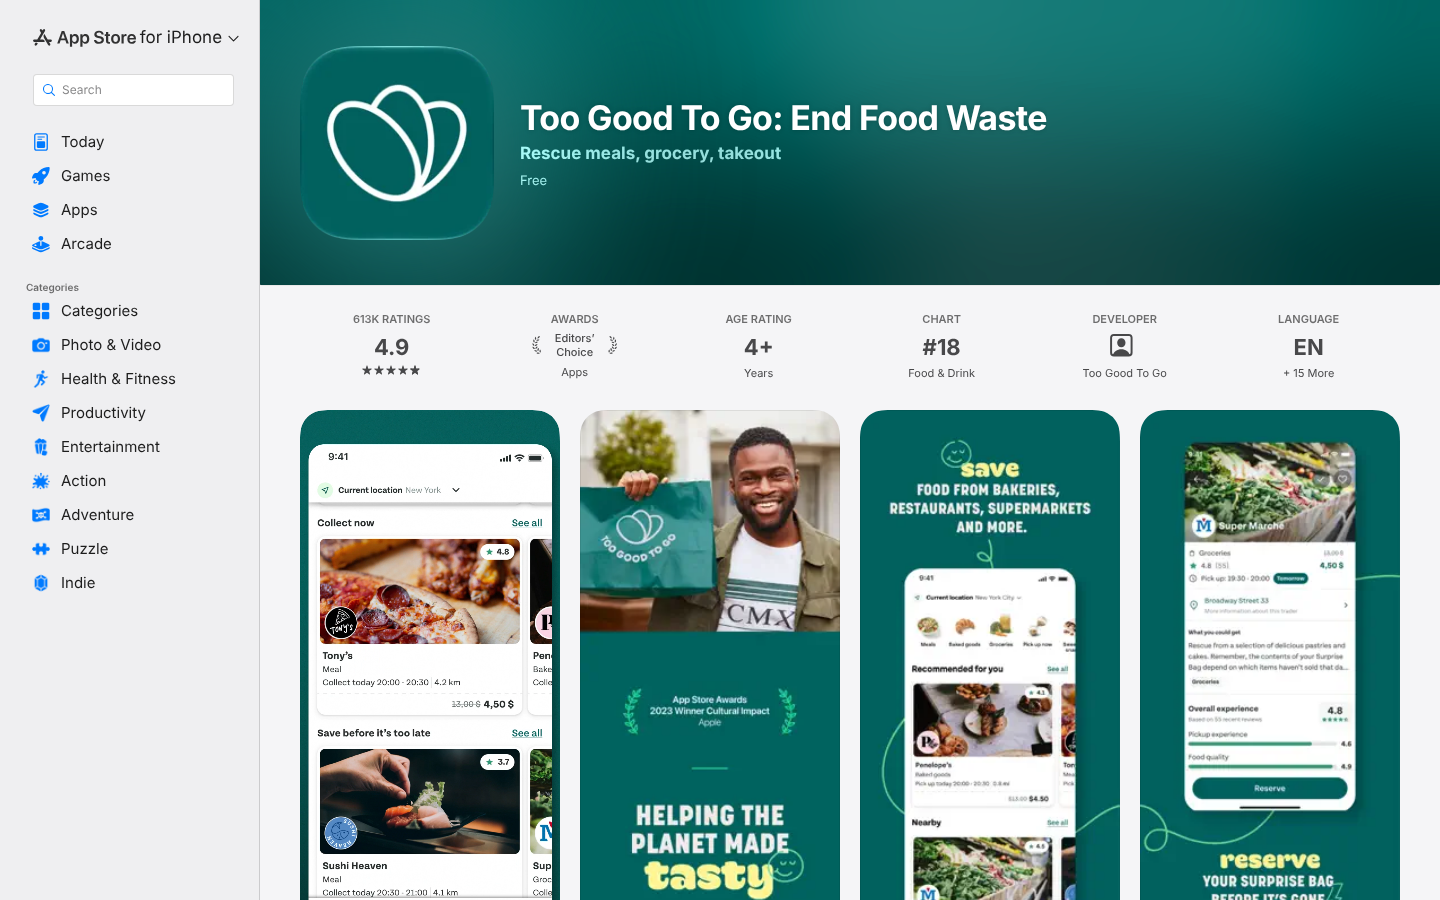
\includegraphics[width=0.92\textwidth]{tgtg.png}
  \caption{Aplikacija Too Good To Go v trgovini App Store: seznam ponudnikov
  s termini prevzema in rezervacija vrečke
  presenečenja~\cite{tgtg-appstore}.}
  \label{fig:tgtg}
\end{figure}

%---------------------------------------------------------------------
\subsection{Primerjava}
%---------------------------------------------------------------------

\begin{table}[H]
  \centering
  \small
  \begin{tabularx}{\textwidth}{X c c c}
    \toprule
    \textbf{Funkcionalnost} & \textbf{Pečjak} & \textbf{Wolt} & \textbf{Too Good To Go} \\
    \midrule
    Spletni katalog izdelkov         & da & da & delno \\
    Prikaz alergenov                 & da & da & ne \\
    Dostava na dom                   & da & da & ne \\
    Osebni prevzem                   & da & da & da \\
    Izbira termina prevzema/dostave  & ni zaznano & da & da (fiksen) \\
    Torte in izdelki po meri         & ne & ne & ne \\
    Naročila za podjetja             & ni zaznano & da & ne \\
    Prodaja ostankov ob koncu dneva  & ne & ne & da \\
    Brez provizije za pekarno        & da & ne & ne \\
    \bottomrule
  \end{tabularx}
  \caption{Primerjava pregledanih rešitev.}
  \label{tab:primerjava}
\end{table}

%=====================================================================
\section{Zaključek}
%=====================================================================

Vse tri rešitve rešujejo del problema, nobena pa ne pokrije potreb manjše
lokalne pekarne, kot je Pekarna Zrno.

\paragraph{Kaj bomo prevzeli.}
\begin{itemize}
  \item od \textbf{Pekarne Pečjak}: pregleden katalog s kategorijami in filtri,
        jasen prikaz sestavin in alergenov ter prag za brezplačno dostavo,
  \item od \textbf{Wolta}: izbiro termina (načrtovano naročilo), prikaz
        delovnega časa in minimalnega zneska ter jasen status naročila,
  \item od \textbf{Too Good To Go}: idejo, da se pecivo, ki ostane ob koncu
        dneva, ponudi po znižani ceni s prevzemom v določenem terminu.
\end{itemize}

\paragraph{Kaj bo naša rešitev naredila drugače ali bolje.}
\begin{itemize}
  \item \textbf{lastna stran pekarne} -- brez provizij posrednikov, s
        poudarkom na lokalni blagovni znamki in zgodbi treh generacij peke,
  \item \textbf{naročilo tort in sladic po meri} (velikost, okus, napis,
        datum prevzema), česar nobena pregledana rešitev ne omogoča,
  \item \textbf{naročila za podjetja in dogodke}, vključno s ponavljajočimi se
        dostavami (npr.\ vsak ponedeljek ob 8:00),
  \item \textbf{prevzem v izbrani poslovalnici} (ena od treh) ob izbranem
        terminu, tudi za svež kruh za naslednji dan,
  \item \textbf{akcija ob koncu dneva}, a z znanimi izdelki in alergeni
        -- namesto vrečke presenečenja,
  \item \textbf{pregled naročil za pekarno} po dnevih in poslovalnicah, da
        lažje načrtuje peko in zmanjša odpadke.
\end{itemize}

%=====================================================================
\begin{thebibliography}{99}\sloppy
%=====================================================================

\bibitem{pecjak-zgodba}
Pekarna Pečjak. \emph{Our Story -- Pekarna Pečjak}.
\url{https://www.pekarna-pecjak.si/en/?p=15599}
(dostopano 24.\,11.\,2026).

\bibitem{pecjak-domov}
Pekarna Pečjak. \emph{Vstopna stran}.
\url{https://www.pekarna-pecjak.si/}
(dostopano 24.\,11.\,2026).

\bibitem{pecjak-trgovina}
Pekarna Pečjak. \emph{Spletna trgovina}.
\url{https://www.pekarna-pecjak.si/trgovina/}
(dostopano 24.\,11.\,2026).

\bibitem{wolt-maribor}
Wolt. \emph{Dostava hrane v Mariboru}.
\url{https://wolt.com/sl/svn/maribor}
(dostopano 24.\,11.\,2026).

\bibitem{wolt-mlinar}
Wolt. \emph{Mlinar Grajski -- Maribor}.
\url{https://wolt.com/sl/svn/maribor/venue/mlinar-grajski}
(dostopano 24.\,11.\,2026).

\bibitem{wolt-mlinar-brand}
Wolt. \emph{Mlinar -- Maribor}.
\url{https://wolt.com/sl/svn/maribor/brand/mlinar}
(dostopano 24.\,11.\,2026).

\bibitem{wolt-storitve}
Wolt. \emph{Storitve: Wolt Drive, Wolt Market, Wolt+, Wolt for Work}.
\url{https://wolt.com/sl/discovery/teta}
(dostopano 24.\,11.\,2026).

\bibitem{wolt-kariere}
Wolt. \emph{Slovenia -- Our history}.
\url{https://careers.wolt.com/en/locations/slovenia}
(dostopano 24.\,11.\,2026).

\bibitem{tgtg-appstore}
Too Good To Go ApS. \emph{Too Good To Go: End Food Waste} (App Store).
\url{https://apps.apple.com/us/app/too-good-to-go-end-food-waste/id1060683933}
(dostopano 24.\,11.\,2026).

\bibitem{tgtg-cz}
Too Good To Go. \emph{Uživatelé Too Good To Go v Česku \dots} (sporočilo za
javnost).
\url{https://www.toogoodtogo.com/cs-cz/press/uzivatele-too-good-to-go-v-cesku-nasli-zpusob-jak-zachranit-nejcasteji-vyhazovane-potraviny}
(dostopano 24.\,11.\,2026).

\bibitem{tgtg-bakery}
Too Good To Go. \emph{Optimise your bakery management}.
\url{https://www.toogoodtogo.com/en-gb/b2b/bakery-management}
(dostopano 24.\,11.\,2026).

\end{thebibliography}

\end{document}
